%%%%%%%%%%%%%%%%%%%%%%%%%%%%%%%%%%%%%%%%%%%%%%%%%%%%%%%%%%%%%%%%
%
%  Template for homework of Introduction to Machine Learning.
%
%  Fill in your name, lecture number, lecture date and body
%  of homework as indicated below.
%
%%%%%%%%%%%%%%%%%%%%%%%%%%%%%%%%%%%%%%%%%%%%%%%%%%%%%%%%%%%%%%%%


\documentclass[11pt,letter,notitlepage]{article}
%Mise en page
\usepackage[left=2cm, right=2cm, lines=45, top=0.8in, bottom=0.7in]{geometry}
\usepackage{fancyhdr}
\usepackage{fancybox}
\usepackage{graphicx}
\usepackage{pdfpages} 
\usepackage{enumitem}
\usepackage{algorithm}
\usepackage{algorithmic}
\renewcommand{\headrulewidth}{1.5pt}
\renewcommand{\footrulewidth}{1.5pt}
\newcommand\Loadedframemethod{TikZ}
\usepackage[framemethod=\Loadedframemethod]{mdframed}

\usepackage{amssymb,amsmath}
\usepackage{amsthm}
\usepackage{thmtools}
\newtheorem{lemma}{Lemma}

\setlength{\topmargin}{0pt}
\setlength{\textheight}{9in}
\setlength{\headheight}{0pt}

\setlength{\oddsidemargin}{0.25in}
\setlength{\textwidth}{6in}

\usepackage{graphicx} % more modern
\usepackage{subfigure}
\usepackage{ctex}
\usepackage{pythonhighlight}

%%%%%%%%%%%%%%%%%%%%%%%%
%%%%%% Define math operator %%%%%
%%%%%%%%%%%%%%%%%%%%%%%%
\DeclareMathOperator*{\argmin}{\bf argmin}
\DeclareMathOperator*{\relint}{\bf relint\,}
\DeclareMathOperator*{\dom}{\bf dom\,}
\DeclareMathOperator*{\intp}{\bf int\,}
%%%%%%%%%%%%%%%%%%%%%%%


\setlength{\topmargin}{0pt}
\setlength{\textheight}{9in}
\setlength{\headheight}{0pt}

\setlength{\oddsidemargin}{0.25in}
\setlength{\textwidth}{6in}
\pagestyle{fancy}
%%%%%%%%%%%%%%%%%%%%%%%%
%% Define the Exercise environment %%
%%%%%%%%%%%%%%%%%%%%%%%%
\mdtheorem[
topline=false,
rightline=false,
leftline=false,
bottomline=false,
leftmargin=-10,
rightmargin=-10
]{exercise}{\textbf{Exercise}}
%%%%%%%%%%%%%%%%%%%%%%%
%% End of the Exercise environment %%
%%%%%%%%%%%%%%%%%%%%%%%


%%%%%%%%%%%%%%%%%%%%%%%%
%% Define the Problem environment %%
%%%%%%%%%%%%%%%%%%%%%%%%
\mdtheorem[
topline=false,
rightline=false,
leftline=false,
bottomline=false,
leftmargin=-10,
rightmargin=-10
]{problem}{\textbf{Problem}}
%%%%%%%%%%%%%%%%%%%%%%%
%% End of the Exercise environment %%
%%%%%%%%%%%%%%%%%%%%%%%

%%%%%%%%%%%%%%%%%%%%%%%
%% Define the Solution Environment %%
%%%%%%%%%%%%%%%%%%%%%%%
\declaretheoremstyle
[
spaceabove=0pt, 
spacebelow=0pt, 
headfont=\normalfont\bfseries,
notefont=\mdseries, 
notebraces={(}{)}, 
headpunct={:\quad}, 
headindent={},
postheadspace={ }, 
postheadspace=4pt, 
bodyfont=\normalfont, 
qed=$\blacksquare$,
preheadhook={\begin{mdframed}[style=myframedstyle]},
	postfoothook=\end{mdframed},
]{mystyle}

\declaretheorem[style=mystyle,title=Solution,numbered=no]{solution}
\mdfdefinestyle{myframedstyle}{%
	topline=false,
	rightline=false,
	leftline=false,
	bottomline=false,
	skipabove=-6ex,
	leftmargin=-10,
	rightmargin=-10}
%%%%%%%%%%%%%%%%%%%%%%%
%% End of the Solution environment %%
%%%%%%%%%%%%%%%%%%%%%%%

%% Homework info.
\newcommand{\posted}{\text{Nov. 5, 2019}}       			%%% FILL IN POST DATE HERE
\newcommand{\due}{\text{Nov. 18, 2019}} 			%%% FILL IN Due DATE HERE
\newcommand{\hwno}{\text{4}} 		           			%%% FILL IN LECTURE NUMBER HERE


%%%%%%%%%%%%%%%%%%%%
%% Put your information here %%
%%%%%%%%%%%%%%%%%%%
\newcommand{\name}{\text{Jiahuan Yu}}  	          			%%% FILL IN YOUR NAME HERE
\newcommand{\id}{\text{PB17121687}}		       			%%% FILL IN YOUR ID HERE
%%%%%%%%%%%%%%%%%%%%
%% End of the student's info %%
%%%%%%%%%%%%%%%%%%%


\newcommand{\proj}[2]{\textbf{P}_{#2} (#1)}
\newcommand{\lspan}[1]{\textbf{span}  (#1)  }
\newcommand{\rank}[1]{ \textbf{rank}  (#1)  }
\newcommand{\RNum}[1]{\uppercase\expandafter{\romannumeral #1\relax}}


\lhead{
	\textbf{\name}
}
\rhead{
	\textbf{\id}
}
\chead{\textbf{
		Homework \hwno
}}


\begin{document}
\vspace*{-4\baselineskip}
\thispagestyle{empty}


\begin{center}
	{\bf\large Introduction to Machine Learning}\\
	{Fall 2019}\\
	University of Science and Technology of China
\end{center}

\noindent
Lecturer: Jie Wang  			 %%% FILL IN LECTURER HERE
\hfill
Homework \hwno
\\
Posted: \posted
\hfill
Due: \due
\\
Name: \name
\hfill
ID: \id
\hfill

\noindent
\rule{\textwidth}{2pt}

\medskip





%%%%%%%%%%%%%%%%%%%%%%%%%%%%%%%%%%%%%%%%%%%%%%%%%%%%%%%%%%%%%%%%
%% BODY OF HOMEWORK GOES HERE
%%%%%%%%%%%%%%%%%%%%%%%%%%%%%%%%%%%%%%%%%%%%%%%%%%%%%%%%%%%%%%%%

\textbf{Notice, }to get the full credits, please show your solutions step by step.

\begin{exercise}[Support Vector Machine (SVM) for Linearly Separable Cases \textnormal{40pts}]
	Given the training sample $\mathcal{D}=\{ (\textbf{x}_i,y_i) \}_{i=1}^n$, where $\textbf{x}_i \in \mathbb{R}^d$ and $y_i \in \{ -1,1 \}$. Let
	\begin{align*}
		\mathcal{D}^+=\{(\textbf{x}_i,y_i)\in\mathcal{D}:y_i=1\},\hspace{5mm}\mathcal{D}^-=\{(\textbf{x}_i,y_i)\in\mathcal{D}:y_i=-1\}.
	\end{align*}
	Assume that $\mathcal{D}^+$ and $\mathcal{D}^-$ are nonempty and the training sample $\mathcal{D}$ is linearly separable. We have shown in class that SVM can be written as
	\begin{align}\label{prob:SVM-1}
		 & \min_{\textbf{w},b}\,\,\cfrac{1}{2}\| \textbf{w} \|^2,                                     \\
		 & \text{ s.t. } \min_i y_{i} ( \langle \textbf{w}, \textbf{x}_i \rangle + b ) = 1. \nonumber
	\end{align}
	Moreover, we further transform the problem in (\ref{prob:SVM-1}) to
	\begin{align}\label{prob:SVM}
		 & \min_{\textbf{w},b}\,\,\cfrac{1}{2}\| \textbf{w} \|^2,                                                   \\
		 & \text{ s.t. }\,\, y_{i} ( \langle \textbf{w}, \textbf{x}_i \rangle + b ) \geq 1, i=1,\ldots,n. \nonumber
	\end{align}
	We denote the feasible set of the problem in (\ref{prob:SVM}) by $$\mathcal{F}=\{(\mathbf{w},b):y_{i} ( \langle \textbf{w}, \textbf{x}_i \rangle + b ) \geq 1, i=1,\ldots,n\}.$$

	\begin{enumerate}
		\item Show that $\mathcal{F}$ is nonempty.
		\item Show that the problem in (\ref{prob:SVM}) admits an optimal solution.
		\item Let $(\textbf{w}^*,b^*)$ be the optimal solution to problem (\ref{prob:SVM}). Show that $\mathbf{w}^*\neq0$.
		\item Show that the problems in (\ref{prob:SVM-1}) and (\ref{prob:SVM}) are equivalent, that is, they share the same set of optimal solutions.
		\item Let $(\textbf{w}^*,b^*)$ be the optimal solution to problem (\ref{prob:SVM}). Show there exist at least one positive sample and one negative sample, respectively, such that the equality holds. In other words, there exist $i,j \in \{ 1,2,\dots,n \}$ such that
		      \begin{align*}
			      1=y_i =  & \langle \textbf{w}^*, \textbf{x}_i \rangle + b^*, \\
			      -1=y_j = & \langle \textbf{w}^*, \textbf{x}_j \rangle + b^*.
		      \end{align*}
		\item Show that the optimal solution to problem (\ref{prob:SVM}) is unique.
		\item Find the dual problem of (\ref{prob:SVM}) and the corresponding optimal conditions.
	\end{enumerate}

\end{exercise}
\begin{solution}
	\begin{enumerate}
		\item % 解的存在性
		      只需证明存在 $(\mathbf{w},b)$ 使得
		      $$\begin{cases}
				      \langle \mathbf{w},\mathbf{x}_i \rangle + b \geq 1 ,  & \text{if $y_i=1$}  \\
				      \langle \mathbf{w},\mathbf{x}_i \rangle + b \leq -1 , & \text{if $y_i=-1$}
			      \end{cases}, i=1,2,\cdots,n$$
		      由于 $\mathbf{D}$ 线性可分,所以一定存在 $\lambda>0$ 和与之对应的 $(\mathbf{w}',b')$, 使得
		      $$\begin{cases}
				      \langle \mathbf{w}',\mathbf{x}_i \rangle + b' \geq \lambda ,  & \text{if $y_i=1$}  \\
				      \langle \mathbf{w}',\mathbf{x}_i \rangle + b' \leq -\lambda , & \text{if $y_i=-1$}
			      \end{cases}, i=1,2,\cdots,n$$
		      以上不等式左右同乘 $\cfrac{1}{\lambda}$, 即可得 $(\cfrac{\mathbf{w}'}{\lambda},\cfrac{b'}{\lambda})$, 即是要求的 $(\mathbf{w},b)$.

		      所以 $\mathcal{F}$ 非空。

		\item % 最优解的存在性
		      若存在最优解,显然最优解必然在 $\|\mathbf{w}\|$ 有限时取到。

		      由于 $\mathcal{F}$ 的定义中,不等式是 $\geq$ 约束的,所以当加入额外约束 $\|\mathbf{w}\|\leq\lambda, \lambda>0$ 产生 $\mathcal{F}'\subset\mathcal{F}$ 时,若 $\mathcal{F}'$ 非空,则 $\mathcal{F}'$ 的边界一定可以取到。

		      又因为 $\|\mathbf{w}\| \geq 0$,即 $\|\mathbf{w}\|$ 存在下确界,所以此下确界一定可以取到(在或不在边界上都可以取到),所以问题 (\ref{prob:SVM}) 一定存在最优解。

		\item 假设 $\mathbf{w}^*=0$, 则
		      $$\begin{cases}
				      b^* \geq 1 ,  & \text{if $y_i=1$}  \\
				      b^* \leq -1 , & \text{if $y_i=-1$}
			      \end{cases}, i=1,2,\cdots,n$$
		      显然这是不可能的,所以 $\mathbf{w}^*\neq 0$.
		\item 设 $(\mathbf{w}^*,b^*)$ 是 (\ref{prob:SVM}) 的最优解,假设
		      $$\min_i y_i (\langle \mathbf{w}, \mathbf{x}_i \rangle +b) = \lambda >1$$
		      则令 $\mathbf{w}'=\cfrac{\mathbf{w}^*}{\lambda}$, $b'=\cfrac{b^*}{\lambda}$, 有
		      $$\min_i y_i (\langle \mathbf{w}', \mathbf{x}_i \rangle +b') =1$$
		      显然 $(\mathbf{w}',b')$ 也是 (\ref{prob:SVM}) 的解,且
		      $$\cfrac{1}{2}\|\mathbf{w}'\|^2=\cfrac{1}{2\lambda^2}\|\mathbf{w}^*\|^2
			      < \cfrac{1}{2}\|\mathbf{w}^*\|^2$$
		      与假设矛盾。所以
		      $$\min_i y_i (\langle \mathbf{w}, \mathbf{x}_i \rangle +b) = 1$$
		      即 (\ref{prob:SVM}) 的最优解也是 (\ref{prob:SVM-1}) 的解。

		      而 (\ref{prob:SVM-1}) 的最优解显然也是 (\ref{prob:SVM}) 的解。

		      所以两者有相同的最优解,即问题 (\ref{prob:SVM-1}) 和问题 (\ref{prob:SVM}) 等价。
		\item 由第 4 小题可知,取最优解时,问题 (\ref{prob:SVM}) 的等号一定能取到。

		      由于对称性,不妨设 $\exists i \in \{1,2,\cdots,n\}$ 使得
		      $$1=y_i=\langle \mathbf{w}^*, \mathbf{x}_i \rangle+b^*$$
		      假设对于 $\forall j \in \{1,2,\cdots,n\}$ 且 $y_j=-1$,有
		      $$\langle \mathbf{w}^*, \mathbf{x}_i \rangle+b^* \leq -\lambda < -1$$
		      令 $b'=b^*+\mu > b^*$, 其中 $0 <\mu<\lambda-1$。 所以
		      $$\begin{cases}
				      \langle \mathbf{w}^*, \mathbf{x}_i \rangle+b' >1 , & \text{if $y_i=1$}  \\
				      \langle \mathbf{w}^*, \mathbf{x}_i \rangle+b' <-1, & \text{if $y_i=-1$}
			      \end{cases}, i=1,2,\cdots,n$$
		      由第 4 小题的结论,$(\mathbf{x}^*,b')$ 不是最优解,所以 $(\mathbf{x}^*,b^*)$ 也不是最优解,矛盾。

		      所以要证的命题成立。
		\item 假设存在两个最优解 $(\mathbf{w}^*_1,b^*_1)$ 和 $(\mathbf{w}^*_2,b^*_2)$.
		      \begin{enumerate}
			      \item 若 $\mathbf{w}_1^* \neq \mathbf{w}_2^*$,则
			            $$\begin{cases}
					            y_i(\langle \mathbf{w}^*_1, \mathbf{x}_i \rangle+b^*_1) \geq 1 \\
					            y_i(\langle \mathbf{w}^*_2, \mathbf{x}_i \rangle+b^*_2) \geq 1
				            \end{cases}, i=1,2,\cdots,n$$
			            两式相加,得
			            $$ y_i \left(\langle \cfrac{\mathbf{w}^*_1+\mathbf{w}^*_2}{2}, \mathbf{x}_i \rangle + \cfrac{b^*_1+b^*_2}{2} \right) \geq 1$$
			            即 $\left( \cfrac{\mathbf{w}^*_1+\mathbf{w}^*_2}{2}, \cfrac{b^*_1+b^*_2}{2} \right)$ 也是一解。
			            又因为
			            $$\|\cfrac{\mathbf{w}^*_1+\mathbf{w}^*_2}{2}\| \leq \cfrac{\|\mathbf{w}^*_1\| + \|\mathbf{w}^*_2\|}{2} = \|\mathbf{w}^*_1\|$$
			            由于 $\mathbf{w}^*_1 \neq \mathbf{w}^*_2$, 所以等号不能取到,所以
			            $$\|\cfrac{\mathbf{w}^*_1+\mathbf{w}^*_2}{2}\| < \|\mathbf{w}^*_1\|$$
			            即 $\left( \cfrac{\mathbf{w}^*_1+\mathbf{w}^*_2}{2}, \cfrac{b^*_1+b^*_2}{2} \right)$ 是比 $( \mathbf{w}^*_1, b_1^*)$ 更优的解,与假设矛盾。
			      \item 若 $\mathbf{w}_1^* = \mathbf{w}_2^* = \mathbf{w}^*$ 且 $b_1^* \neq b_2^*$, 不妨设 $b_1^* < b_2^*$.

			            由第 4 小题可知,取最优解时,问题 (\ref{prob:SVM}) 的等号一定能取到。

			            由于对称性($y_i=-1$ 的情况类似处理),不妨设 $\exists i \in \{1,2,\cdots,n\}$ 使得
			            $$1=y_i=\langle \mathbf{w}^*, \mathbf{x}_i \rangle+b_2^*$$
			            那么
			            $$\langle \mathbf{w}^*, \mathbf{x}_i \rangle+b_1^*
				            < \langle \mathbf{w}^*, \mathbf{x}_i \rangle+b_2^*
				            =1$$
			            $$y_i ( \langle \mathbf{w}^*, \mathbf{x}_i \rangle+b_1^*)<1$$
			            则 $(\mathbf{w}^*_1,b^*_1)$ 不是问题 (\ref{prob:SVM}) 的解,矛盾。
		      \end{enumerate}


		      所以解是唯一的。
		\item 引入 Lagrange 乘子 $\alpha_i \geq 0, i=1,2,\cdots,n$.

		      问题 (\ref{prob:SVM}) 的对偶问题可写为
		      $$\begin{aligned}
				       & L(\mathbf{x},b,\mathbf{\alpha}) = \cfrac{1}{2}\|\mathbf{w}\|^2 + \sum_{i=1}^{n}{\alpha_i \left( 1-y_i(\langle \mathbf{w},\mathbf{x}_i \rangle+b) \right)} \\
				       & \max_{\mathbf{\alpha}}\min_{\mathbf{w},b}L(\mathbf{x},b,\alpha)
			      \end{aligned}$$
		      对 $L$ 求导
		      $$\begin{aligned}
				      \nabla_{\mathbf{w}} L(\mathbf{x},b,\mathbf{\alpha}) & = \mathbf{w}-\sum_{i=1}^{n}{\alpha_i y_i \mathbf{x}_i} & =0 \\
				      \nabla_b L(\mathbf{x},b,\mathbf{\alpha})            & = -\sum_{i=1}^{n}{\alpha_i y_i}                        & =0
			      \end{aligned}$$
		      于是可得对偶问题
		      $$\begin{aligned}
				      \max_{\mathbf{\alpha}} & \left( \sum_{i=1}^{n}{\mathbf{\alpha}_i} - \cfrac{1}{2} \sum_{i=1}^{n}{\sum_{i=1}^{n}{\alpha_i \alpha_j y_i y_j \mathbf{x}_i^\top \mathbf{x}_j }}\right) \\
				      \text{s.t.}            & \sum_{i=1}^{n}{\alpha_i y_i}=0                                                                                                                           \\
				                             & \alpha_i \geq 0, i=1,2,\cdots,n
			      \end{aligned}$$
	\end{enumerate}
\end{solution}

\newpage
\begin{exercise}[Visualization Lemma]
	Consider the primal problem as follows.
	\begin{align}\label{prob:primal-vec}
		\min_{\mathbf{x}}\, & f(\mathbf{x})                \\ \nonumber
		{\rm s.t.}\,        & \mathbf{g}(\mathbf{x})\leq0, \\ \nonumber
		                    & \mathbf{h}(\mathbf{x})=0,    \\ \nonumber
		                    & \mathbf{x}\in X,
	\end{align}
	where $\mathbf{x}\in\mathbb{R}^n$, $f:\mathbb{R}^n\rightarrow\mathbb{R}$, $\mathbf{g}:\mathbb{R}^n\rightarrow\mathbb{R}^m$, $\mathbf{h}:\mathbb{R}^n\rightarrow\mathbb{R}^p$, and $X\subseteq\mathbb{R}^n$. The functions $f$, $\mathbf{g}$, and $\mathbf{h}$ are continuously differentiable.

	The Lagrangian $L:\mathbb{R}^n\times \mathbb{R}^m\times \mathbb{R}^p\rightarrow\mathbb{R}$ associated with the problem in (\ref{prob:primal-vec}) takes the form of
	\begin{align}\label{def:Lagrangian}
		L(\mathbf{x},\lambda,\mu)=f(\mathbf{x})+\sum_{i=1}^m\lambda_ig_i(\mathbf{x})+\sum_{i=1}^p\mu_ih_i(\mathbf{x}).
	\end{align}

	Let
	\begin{align}\label{def:image-set}
		\mathbb{R}^{m+p+1}\supseteq S=\{(\mathbf{g}(\mathbf{x}),\mathbf{h}(\mathbf{x}),f(\mathbf{x})):\mathbf{x}\in X\}.
	\end{align}

	Show that the results as follows (hint: see Fig. \ref{fig:visualization-lemma}).

	\begin{lemma}
		\textbf{\textup {Visualization Lemma}}
		\begin{enumerate}
			\item The hyperplane with normal $(\lambda,\mu,1)$ that passes through a vector $(\mathbf{g}(\mathbf{x}),\mathbf{h}(\mathbf{x}),f(\mathbf{x}))$ intercepts the vertical axis $\{(\mathbf{0},z):z\in\mathbb{R}\}$ at the level $L(\mathbf{x},\lambda,\mu)$.

			\item Among all hyperplanes with normal $(\lambda,\mu,1)$ that contains in their positive halfspace the set $S$ defined in (\ref{def:image-set}), the highest attained level of interception of the vertical axis is $\inf_{\mathbf{x}\in X}\,L(\mathbf{x},\lambda,\mu)$.

			\item $(\lambda^*,\mu^*)$ is a geometric multiplier if and only if $\lambda^*\geq0$ and among all hyperplanes with normal $(\lambda^*,\mu^*,1)$ that contain in their positive halfspace the set $S$, the highest attained level of of interception of the vertical axis is $f^*$, where
			      \begin{align*}
				      f^*=\min\{f(\mathbf{x}):\mathbf{g}(\mathbf{x})\leq0,\mathbf{h}(\mathbf{x})=0,\mathbf{x}\in X\}.
			      \end{align*}
		\end{enumerate}
	\end{lemma}
\end{exercise}
\begin{figure}[!h]
	\centering{
		\subfigure[] { \label{fig:geometric-multiplier-0}
			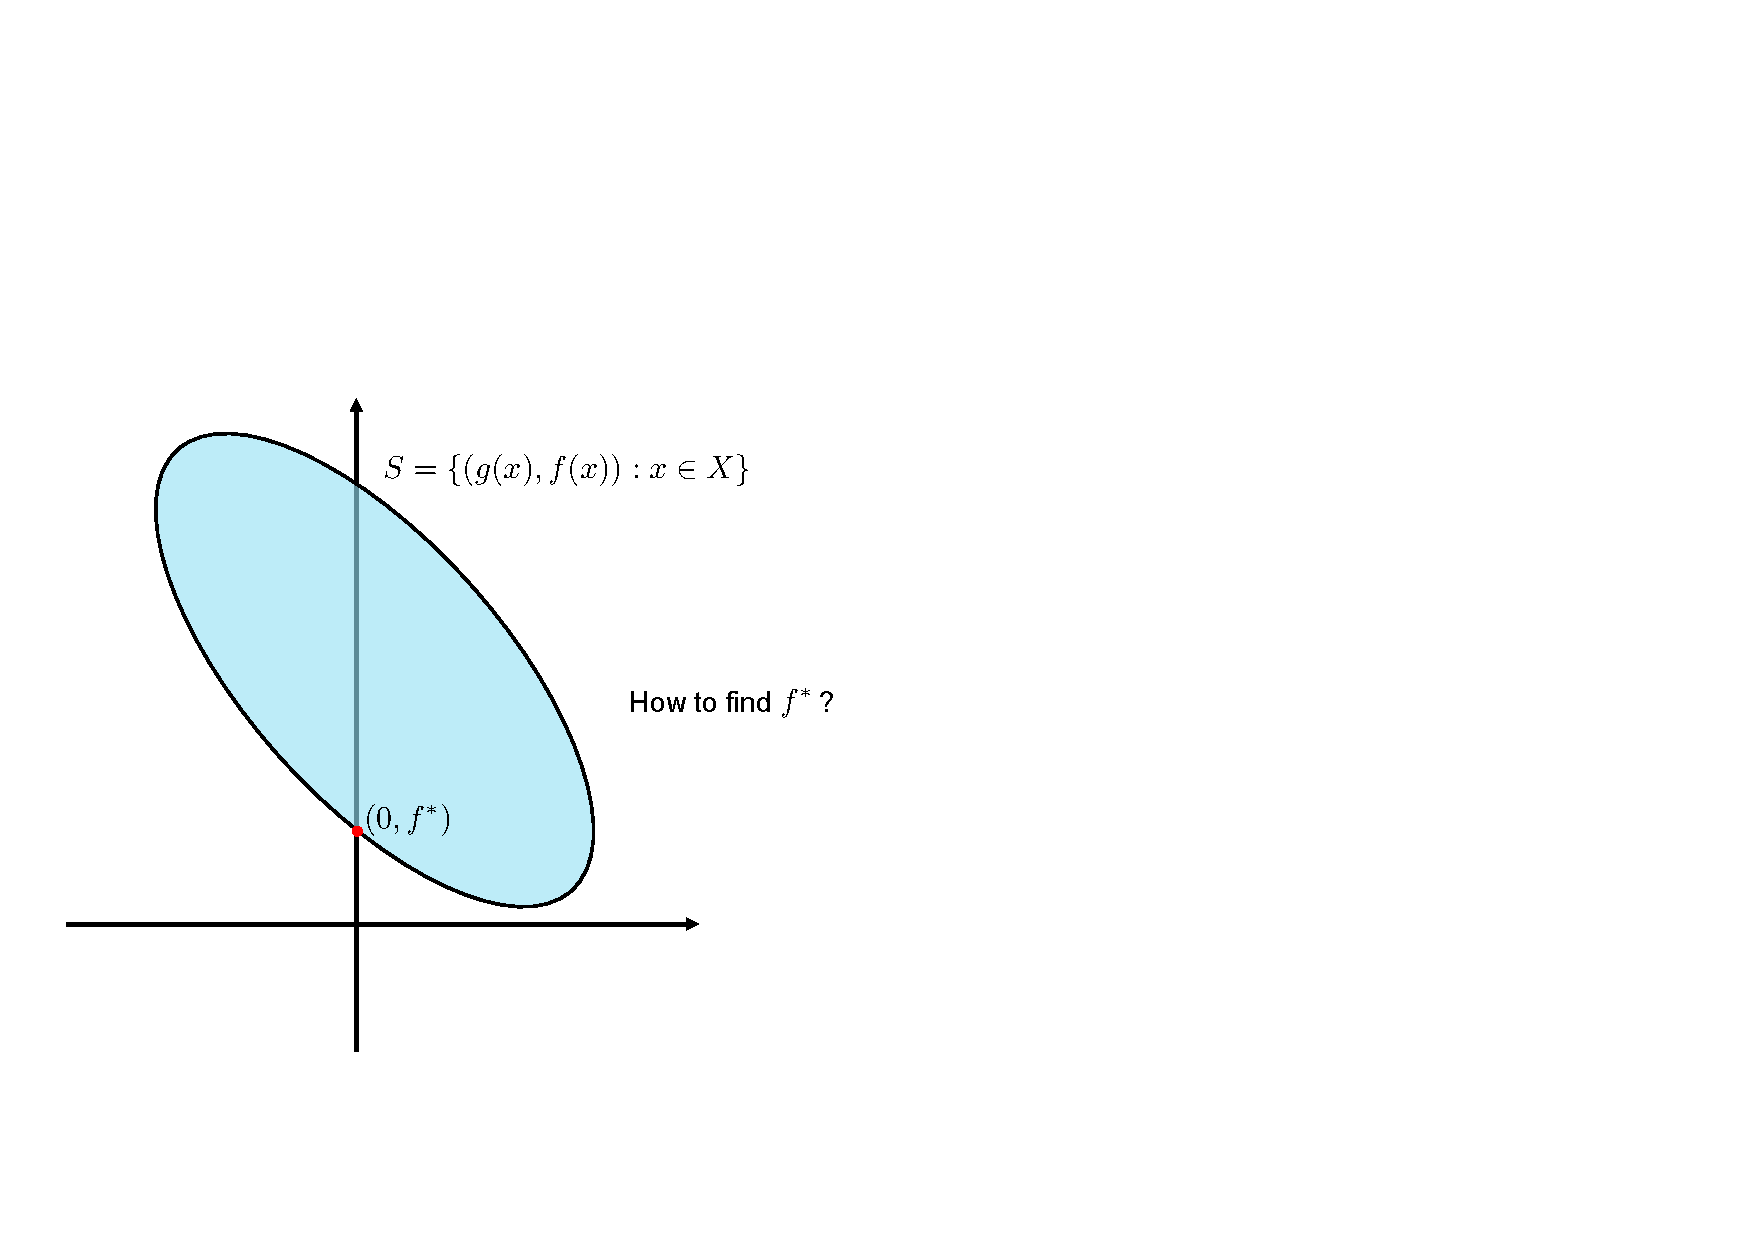
\includegraphics[width=0.45\columnwidth]{figures/geometric-multipliers-0.pdf}
		}
		\subfigure[] { \label{fig:geometric-multiplier-1}
			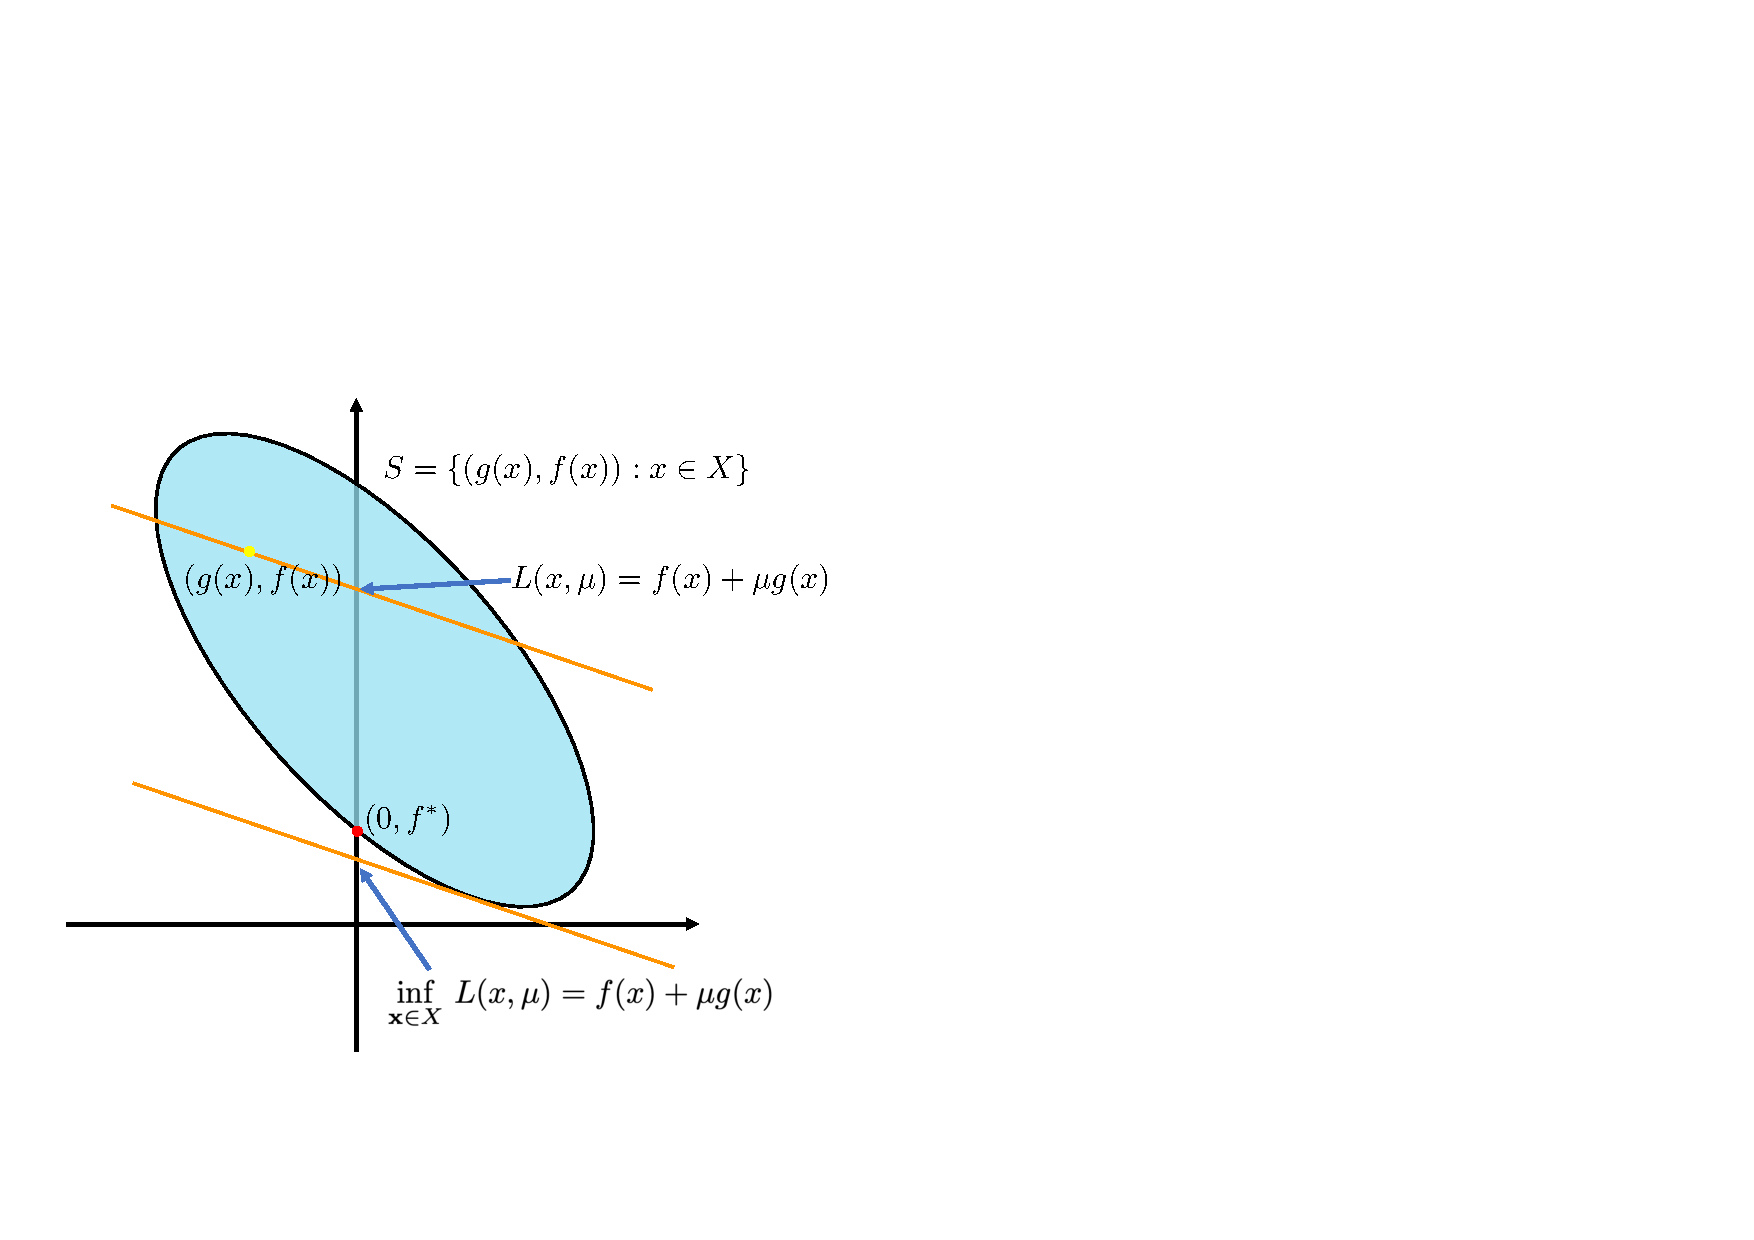
\includegraphics[width=0.45\columnwidth]{figures/geometric-multipliers-1.pdf}
		}
	}
	\caption{Illustration of the visualization lemma with one inequality constraint.}
	\label{fig:visualization-lemma}
\end{figure}

\begin{solution}
	\begin{enumerate}
		\item 设空间坐标为 $(\mathbf{w},\mathbf{v},z), \mathbf{w}\in\mathbb{R}^m, \mathbf{v}\in\mathbb{R}^p$.

		      因为超平面有法向量 $(\mathbf{\lambda,\mathbf{\mu}},1)$, 所以其方程可写为
		      $$C=\langle \mathbf{\lambda},\mathbf{w} \rangle + \langle \mathbf{\mu},\mathbf{v} \rangle + z$$
		      因为超平面过 $(\mathbf{g}(\mathbf{x}),\mathbf{h}(\mathbf{x}),f(\mathbf{x}))$, 令
		      $$\langle \mathbf{\lambda},\mathbf{w} \rangle + \langle \mathbf{\mu},\mathbf{v} \rangle + z
			      = \langle \mathbf{\lambda},\mathbf{g}(\mathbf{x}) \rangle + \langle \mathbf{\mu},\mathbf{h}(\mathbf{x}) \rangle + f(\mathbf{x})$$
		      当 $\mathbf{w}=\mathbf{0}, \mathbf{v}=\mathbf{0}$ 时,可得
		      $$z = \langle \mathbf{\lambda},\mathbf{g}(\mathbf{x}) \rangle + \langle \mathbf{\mu},\mathbf{h}(\mathbf{x}) \rangle + f(\mathbf{x})
			      = L( \mathbf{x},\mathbf{\lambda}, \mathbf{\mu} )$$
		      得证。
		\item 同上题,超平面 $P$ 的方程可写为
		      $$C=\langle \mathbf{\lambda},\mathbf{w} \rangle + \langle \mathbf{\mu},\mathbf{v} \rangle + z$$

		      现设此超平面使得 $S$ 中的所有点都在其划分出的正半空间中,即
		      $$\langle \mathbf{\lambda},\mathbf{g}(\mathbf{x}) \rangle + \langle \mathbf{\mu},\mathbf{h}(\mathbf{x}) \rangle + f(\mathbf{x}) \geq C, \forall (\mathbf{g}(\mathbf{x}),\mathbf{h}(\mathbf{x}),f(\mathbf{x})) \in S$$

		      令 $\mathbf{w}=\mathbf{g}(\mathbf{x})=\mathbf{0}, \mathbf{v}=\mathbf{h}(\mathbf{x})=\mathbf{0}$.
		      此时 $f(\mathbf{x})$ 即为过 $(\mathbf{g}(\mathbf{x}),\mathbf{h}(\mathbf{x}),f(\mathbf{x}))$ 且与 $P$ 平行的超平面的纵截距 $z_0'$,同时 $C$ 也为超平面 $P$ 的纵截距 $z_0$.
		      $$z_0'=f(\mathbf{x}) \geq C = z_0$$

		      由上题可知
		      $$z_0'=L(\mathbf{x},\lambda,\mu)$$

		      所以由 $\mathbf{x}$ 和 $C$ 的任取性,可知
		      $$\inf_{\mathbf{x}\in X} z_0'
			      =\inf_{\mathbf{x}\in X}\,L(\mathbf{x},\lambda,\mu)
			      \geq C$$
		      所以 $\max{C}=\inf_{\mathbf{x}\in X}\,L(\mathbf{x},\lambda,\mu)$

		\item \begin{enumerate}
			      \item 必要性:设 $(\lambda^*,\mu^*)$ 是 geometric multiplier.

			            根据定义有 $\lambda^*\geq0$, 且 $f^*=\inf_{\mathbf{x}\in X} L(\mathbf{x},\lambda^*,\mu^*)$.

			            由第 2 小题可知 $f^*$ 即是法向量为 $(\lambda^*,\mu^*,1)$ 的超平面的最高纵截距。

			            下证 $f^*=\min\{f(\mathbf{x}):\mathbf{g}(\mathbf{x})\leq0,\mathbf{h}(\mathbf{x})=0,\mathbf{x}\in X\}$.

			            假设 $S$ 在 $\mathbf{g}(\mathbf{x})\geq0,\mathbf{h}(\mathbf{x})=0$ 的空间内存在 $f'<f^*$ 且 $\mathbf{g}(\mathbf{x})\neq 0$.

			            设法向量为 $(\lambda^*,\mu^*,1)$ 且过 $(\mathbf{g}(\mathbf{x}'),\mathbf{0},f')$ 的超平面的纵截距为 $f_0'$.

			            因为 $\lambda^*\geq0$, 所以
			            $$f_0'=f'+\langle \lambda^*,\mathbf{g}(\mathbf{x}')-\mathbf{0} \rangle \leq f'<f^*$$

			            所以 $f_0'$ 是一个更小的截距,矛盾。

			            所以 $f^*=\min\{f(\mathbf{x}):\mathbf{g}(\mathbf{x})\leq0,\mathbf{h}(\mathbf{x})=0,\mathbf{x}\in X\}$.

			      \item 充分性:设 $f^*$ 即是法向量为 $(\lambda^*,\mu^*,1)$ 的超平面的最高纵截距,且 $\lambda^*\geq0$.

			            由第二小题可知
			            $$f^*=\inf_{\mathbf{x}\in X} L(\mathbf{x},\lambda^*,\mu^*)$$
			            又因为 $\lambda^*\geq0$, 所以 $(\lambda^*,\mu^*)$ 是 geometric multiplier.
		      \end{enumerate}

	\end{enumerate}
\end{solution}


\newpage
\begin{exercise}[Geometric Multiplier]
	Let $(\lambda^*,\mu^*)$ be a geometric multiplier. Show that $\mathbf{x}^*$ is a global minimum of the primal problem (\ref{prob:primal-vec}) if and only if $\mathbf{x}^*$ is feasible and
	\begin{align*}
		 & \mathbf{x}^*\in\argmin_{\mathbf{x}\in X}\,L(\mathbf{x},\lambda^*,\mu^*), \\
		 & \lambda_i^*g_i(\mathbf{x}^*)=0,\,i=1,\ldots,m.
	\end{align*}
\end{exercise}

\begin{solution}
	\begin{enumerate}
		\item 充分性:设 $\mathbf{x}^*$ 是可行解且
		      \begin{align*}
			       & \mathbf{x}^*\in\argmin_{\mathbf{x}\in X}\,L(\mathbf{x},\lambda^*,\mu^*), \\
			       & \lambda_i^*g_i(\mathbf{x}^*)=0,\,i=1,\ldots,m.
		      \end{align*}
		      geometric multiplier 的定义要求
		      $$f(\mathbf{x}^*)=f^*=\inf_{\mathbf{x}\in X}\ L(\mathbf{x},\lambda^*,\mu^*)$$
		      所以当 $\mathbf{x}^*\in\argmin_{\mathbf{x}\in X}\,L(\mathbf{x},\lambda^*,\mu^*)$ 时,$\mathbf{x}^*$ 是全局最小点。
		\item  必要性:设 $\mathbf{x}^*$ 是问题 (\ref{prob:primal-vec}) 的最小值,即 $f(\mathbf{x}^*)=f^*$

		      由 geometric multiplier 的定义可知
		      $$f^*=\inf_{\mathbf{x}\in X}\ L(\mathbf{x},\lambda^*,\mu^*)
			      =\inf_{\mathbf{x}\in X}\ \left( f(\mathbf{x}) +\langle \mathbf{\lambda}^*,\mathbf{g}(\mathbf{x}) \rangle + \langle \mathbf{\mu}^*,\mathbf{h}(\mathbf{x}) \rangle \right) $$
		      由问题 (\ref{prob:primal-vec}) 可知取最小值时
		      $$\mathbf{h}(\mathbf{x^*})=0$$
		      $$\langle \mathbf{\mu}^*,\mathbf{h}(\mathbf{x^*}) \rangle=0$$
		      所以
		      $$f^*=\inf_{\mathbf{x}\in X}\ \left( f(\mathbf{x}) +\langle \mathbf{\lambda}^*,\mathbf{g}(\mathbf{x}) \rangle \right)
			      = \inf_{\mathbf{x}\in X}\ f(\mathbf{x}) $$
		      显然有
		      $$\langle \mathbf{\lambda}^*,\mathbf{g}(\mathbf{x^*})\rangle =0$$
		      同时,因为
		      $$f(\mathbf{x}^*)=f^*=\inf_{\mathbf{x}\in X}\ L(\mathbf{x},\lambda^*,\mu^*)$$
		      所以有
		      $$\mathbf{x}^*\in\argmin_{\mathbf{x}\in X}\,L(\mathbf{x},\lambda^*,\mu^*)$$
	\end{enumerate}
\end{solution}

\newpage
\begin{exercise}[Lagrange Dual Problem]
	Consider the primal problem (\ref{prob:primal-vec}) and the Lagrangian (\ref{def:Lagrangian}). We define the dual function for $(\lambda,\mu)\in\mathbb{R}^{m+p}$ by
	\begin{align*}
		q(\lambda,\mu)=\inf_{\mathbf{x}\in X}\,L(\mathbf{x},\lambda,\mu).
	\end{align*}
	The domain of $q$ is
	\begin{align*}
		\dom(q)=\{(\lambda,\mu):q(\lambda,\mu)>-\infty\}.
	\end{align*}
	The dual problem is
	\begin{align*}
		\sup\,       & q(\lambda,\mu), \\
		\mbox{s.t. } & \lambda\geq0.
	\end{align*}
	\begin{enumerate}
		\item Show that $\dom(q)$ is convex.
		\item Show that $-q(\lambda,\mu)$ is a convex function.
	\end{enumerate}
\end{exercise}

\begin{solution}
	\begin{enumerate}
		\item 由 2.2 小题可知,要保证 $\inf_{\mathbf{x}\in X}\,L(\mathbf{x},\lambda,\mu)$ 存在,只需要保证存在一个由 $(\lambda,\mu)$ 和 $C$ 确定的超平面使得 $S$ 的所有点都在此超平面划分出的正半空间上。

		      因为超平面的方程 $C=\langle \mathbf{\lambda},\mathbf{w} \rangle + \langle \mathbf{\mu},\mathbf{v} \rangle + z$ 中,$z$ 前的系数不为 0,所以超平面不可能和 $z$ 轴平行。

		      所以只要 $S$ 有下界,$\inf_{\mathbf{x}\in X}\,L(\mathbf{x},\lambda,\mu)$ 即存在。

		      $S$ 是否存在下界只和 $f(\mathbf{x}),\mathbf{g}({\mathbf{x}}),\mathbf{h}(\mathbf{x})$ 有关,和 $\lambda,\mu$ 无关。

		      所以只要 $\dom (q) \neq \emptyset$, 就有 $\dom (q)=\mathbb{R}^2$, 是凸集。
		\item 设 $(\lambda_1,\mu_1), (\lambda_2,\mu_2) \in \dom (q)$, $\theta \in [0,1]$.
		      所以
		      $$\begin{aligned}
				           & -\theta q(\lambda_1,\mu_1) - (1-\theta) q(\lambda_2,\mu_2)                                                                                                                                                                                                                                                                   \\
				      =    & -\theta \inf_{\mathbf{x}\in X} L(\mathbf{x},\lambda_1,\mu_1) - (1-\theta) \inf_{\mathbf{x}\in X} L(\mathbf{x},\lambda_2,\mu_2)                                                                                                                                                                                               \\
				      =    & -\left[ \inf_{\mathbf{x}\in X} \theta L(\mathbf{x},\lambda_1,\mu_1) + \inf_{\mathbf{x}\in X} (1-\theta) L(\mathbf{x},\lambda_2,\mu_2) \right]                                                                                                                                                                                \\
				      \geq & -\inf_{\mathbf{x}\in X} \left[ \theta L(\mathbf{x},\lambda_1,\mu_1) +(1-\theta) L(\mathbf{x},\lambda_2,\mu_2)\right]                                                                                                                                                                                                         \\
				      =    & -\inf_{\mathbf{x}\in X} \left[ \theta \left( f(\mathbf{x}) + \langle \lambda_1, \mathbf{g}(\mathbf{x}) \rangle + \langle \mu_1, \mathbf{h}(\mathbf{x}) \rangle \right) + (1-\theta) \left( f(\mathbf{x}) + \langle \lambda_2, \mathbf{g}(\mathbf{x}) \rangle + \langle \mu_2, \mathbf{h}(\mathbf{x}) \rangle \right) \right] \\
				      =    & -\inf_{\mathbf{x}\in X} \left[ f(\mathbf{x}) + \langle \theta\lambda_1+(1-\theta)\lambda_2, \mathbf{g}(\mathbf{x}) \rangle + \langle \theta\mu_1+(1-\theta)\mu_2, \mathbf{h}(\mathbf{x}) \rangle  \right]                                                                                                                    \\
				      =    & -\inf_{\mathbf{x}\in X} L(\mathbf{x},\theta\lambda_1+(1-\theta)\lambda_2,\theta\mu_1+(1-\theta)\mu_2)                                                                                                                                                                                                                        \\
				      =    & -q (\theta\lambda_1+(1-\theta)\lambda_2,\theta\mu_1+(1-\theta)\mu_2)
			      \end{aligned}$$
		      所以 $-q(\lambda,\mu)$ 是凸函数。
	\end{enumerate}
\end{solution}


\newpage
\begin{exercise}[Duality Gap]
	Duality gap is defined by
	\begin{align*}
		f^*-q^*.
	\end{align*}
	Show that the following results hold.
	\begin{enumerate}
		\item If there is no duality gap, the set of geometric multipliers is equal to the set of optimal dual solutions.
		\item If there is duality gap, the set of geometric multipliers is empty.
	\end{enumerate}
\end{exercise}

\begin{solution}
	\begin{enumerate}
		\item 设 $q^*=q(\lambda',\mu')$. 设 $(\lambda^*,\mu^*)$ 是 geometric multiplier, 于是有
		      $$q^*=q(\lambda',\mu') \leq q(\lambda^*,\mu^*)
			      =\inf_{\mathbf{x}\in X}\ L(\mathbf{x},\lambda^*,\mu^*)=f^*$$
		      因为 $q^*=f^*$, 所以
		      $$q(\lambda',\mu') = q(\lambda^*,\mu^*)$$
		      即 geometric multiplier 都是对偶问题的最优解。

		      同时,当 $\lambda \geq 0, \mathbf{g}(\mathbf{x})\leq0, \mathbf{h}(\mathbf{x})=0$ 时
		      $$\begin{aligned}
				      q^*
				       & =q(\lambda',\mu')                                                                                                \\
				       & =\inf_{\mathbf{x}\in X}\ L(\mathbf{x},\lambda',\mu')                                                             \\
				       & \leq f(\mathbf{x})+\langle \lambda',\mathbf{g}(\mathbf{x}) \rangle + \langle \mu',\mathbf{h}(\mathbf{x}) \rangle \\
				       & \leq f(\mathbf{x})
			      \end{aligned}$$
		      令 $\mathbf{x}=\mathbf{x}^*$, 因为 $q^*=f^*$, 所以
		      $$\begin{aligned}
				      q^*
				       & =q(\lambda',\mu')                                                                                                   \\
				       & =\inf_{\mathbf{x}\in X}\ L(\mathbf{x},\lambda',\mu')                                                                \\
				       & = f(\mathbf{x}^*)+\langle \lambda',\mathbf{g}(\mathbf{x}^*) \rangle + \langle \mu',\mathbf{h}(\mathbf{x}^*) \rangle \\
				       & = f^*
			      \end{aligned}$$
		      由 geometric multiplier 的定义可知 $(\lambda',\mu')$ 为geometric multiplier. 即对偶问题的最优解是 geometric multiplier.

		      综上,当 $f^*=q^*$ 时,geometric multiplier 的集合等于对偶问题的最优解集合。
		\item 假设存在 geometric multiplier $(\lambda^*,\mu^*)$.
		      所以
		      $$q^* <q(\lambda^*,\mu^*)=\inf_{\mathbf{x}\in X} L(\mathbf{x},\lambda^*,\mu^*)=f^*$$
		      同时
		      $$q^*=\sup \inf_{\mathbf{x}\in X} L(\mathbf{x},\lambda,\mu)
			      =\sup\ q(\lambda,\mu)$$
		      所以
		      $$\sup\ q(\lambda,\mu) < q(\lambda^*,\mu^*)$$
		      矛盾。所以不存在 geometric multiplier.
	\end{enumerate}
\end{solution}


\newpage
\begin{exercise}[Optimality Conditions]
	Show that a pair $\mathbf{x}^*$ and $(\lambda^*,\mu^*)$ is an optimal solution and geometric multiplier pair if and only if
	\begin{align}\label{cond:primal-feasibility}
		\mathbf{x}^*\in X,\,\mathbf{g}(\mathbf{x}^*)\leq0,\mathbf{h}(\mathbf{x}^*)=0,\hspace{18.5mm}(\mbox{\textup{Primal Feasibility}}), & \\ \label{cond:dual-feasibility}
		\lambda^*\geq0,\hspace{22mm}(\mbox{\textup{Dual Feasibility}}),                                                                   & \\ \label{cond:lagrangian-optimality}
		\mathbf{x}^*\in\argmin_{\mathbf{x}\in X}\,L(\mathbf{x},\lambda^*,\mu^*),\hspace{10mm}(\mbox{\textup{Lagrangian Optimality}}),     & \\ \label{cond:complementary-slackness}
		\lambda^*_ig_i(\mathbf{x}^*)=0,\,i=1,\ldots,m,\hspace{5mm}(\mbox{\textup{Complementary Slackness}}).                              &
	\end{align}
\end{exercise}

\begin{solution}
	\begin{enumerate}
		\item 必要性:设 $\mathbf{x}^*$ 是最优解并且 $(\lambda^*,\mu^*)$ 是 geometric multiplier.

		      由 2.3 小题,(\ref{cond:primal-feasibility}) 和 (\ref{cond:dual-feasibility}) 成立。

		      由第 3 小题,(\ref{cond:lagrangian-optimality}) 和 (\ref{cond:complementary-slackness}) 成立。

		\item 充分性:设条件 (\ref{cond:primal-feasibility}) (\ref{cond:dual-feasibility}) (\ref{cond:lagrangian-optimality}) (\ref{cond:complementary-slackness}) 成立。

		      因为
		      $$\mathbf{x}^*\in\argmin_{\mathbf{x}\in X}\,L(\mathbf{x},\lambda^*,\mu^*)$$
		      所以
		      $$f^*=f(\mathbf{x}^*)= \inf_{\mathbf{x}\in X} L(\mathbf{x},\lambda^*,\mu^*)$$
		      又因为 $\lambda^* \geq 0$, 所以 $(\lambda^*,\mu^*)$ 是 geometric multiplier.

		      再由第 3 小题,$\mathbf{x}^*$ 是全局最小点,即最优解。
	\end{enumerate}
\end{solution}

\newpage
\begin{exercise}[Saddle Point Interpretation]
	Show that a pair $\mathbf{x}^*$ and $(\lambda^*,\mu^*)$ is an optimal solution-geometric multiplier pair if and only if $\mathbf{x}^*\in X$, $\lambda^*\geq0$, and $(\mathbf{x}^*,\lambda^*,\mu^*)$ is a saddle point of the Lagrangian, in the sense that
	\begin{align}\label{cond:saddle-Lagrangian}
		L(\mathbf{x}^*,\lambda,\mu)\leq L(\mathbf{x}^*,\lambda^*,\mu^*)\leq L(\mathbf{x},\lambda^*,\mu^*),\,\forall\,\mathbf{x}\in X,\,\lambda\geq0.
	\end{align}
\end{exercise}

\begin{solution}
	% 由第 6 小题可知
	\begin{enumerate}
		\item 必要性:设 $\mathbf{x}^*$ 是最优解,$(\lambda^*,\mu^*)$ 是 geometric multiplier.

		      由第 6 题可知
		      $$\mathbf{x}^* \in \argmin_{\mathbf{x}\in X} L(\mathbf{x},\lambda^*,\mu^*)$$
		      所以有
		      $$L(\mathbf{x}^*,\lambda^*,\mu^*) \leq L(\mathbf{x},\lambda^*,\mu^*)$$
		      由 2.3 小题可知,$(\lambda^*,\mu^*)$ 是 geometric multiplier 时,超平面的纵截距 $L(\mathbf{x},\lambda^*,\mu^*)$ 是最大值。所以
		      $$L(\mathbf{x}^*,\lambda,\mu) \leq L(\mathbf{x},\lambda^*,\mu^*)$$
		\item 充分性:设 $L(\mathbf{x}^*,\lambda,\mu)\leq L(\mathbf{x}^*,\lambda^*,\mu^*)\leq L(\mathbf{x},\lambda^*,\mu^*),\,\forall\,\mathbf{x}\in X,\,\lambda\geq0$
		      因为
		      $$L(\mathbf{x}^*,\lambda^*,\mu^*) \leq L(\mathbf{x},\lambda^*,\mu^*)$$
		      所以
		      $$\mathbf{x}^*=\argmin_{\mathbf{x}\in X} L(\mathbf{x},\lambda^*,\mu^*)$$
		      所以 $\mathbf{x}^*$ 是最优解。同时又有
		      $$f^*=f(\mathbf{x}^*)=\inf_{\mathbf{x}\in X} L(\mathbf{x},\lambda^*,\mu^*)$$
		      且 $\lambda \geq0$, 可知 $(\lambda^*,\mu^*)$ 是 geometric multiplier.
	\end{enumerate}
\end{solution}

\newpage
\begin{exercise}
	Recall that the soft margin SVM takes the form of
	\begin{align}\label{prob:soft-SVM}
		\min_{\mathbf{w},b,\xi}\, & \cfrac{1}{2}\|\mathbf{w}\|^2+C\sum_{i=1}^n\xi_i,                          \\ \nonumber
		{\rm s.t.\,}              & \,y_i(\langle\mathbf{w},\mathbf{x}_i\rangle+b)\geq1-\xi_i,i=1,\ldots,n, & \\ \nonumber
		                          & \,\xi_i\geq0,\,i=1,\ldots,n,
	\end{align}
	where $C>0$.
	The corresponding dual problem is
	\begin{align}\label{prob:dual-soft-SVM}
		\min_{\alpha}\, & \cfrac{1}{2}\sum_{i=1}^n\sum_{j=1}^n\,\alpha_i\alpha_jy_iy_j\langle\mathbf{x}_i,\mathbf{x}_j\rangle-\sum_{i=1}^n\alpha_i \\\nonumber
		\mbox{s.t. }\,  & \sum_{i=1}^n\alpha_iy_i=0,                                                                                               \\\nonumber
		                & \alpha_i\in[0,C],i=1,\ldots,n.
	\end{align}
	\begin{enumerate}
		\item Show that the problems (\ref{prob:soft-SVM}) and (\ref{prob:dual-soft-SVM}) always admit optimal solutions.

		\item Suppose that the training data consists of two data instances $x_1=1$ and $x_2=-1$, and the corresponding labels are $y_1=1$ and $y_2=-1$.
		      \begin{enumerate}
			      \item Please solve problem (\ref{prob:SVM}) and find the primal and dual optimal solutions.
			      \item Please solve problem (\ref{prob:soft-SVM}) with $C<\cfrac{1}{2}$ and find the primal and dual optimal solutions.
		      \end{enumerate}

		\item Suppose that the training data consists of four data instances: $\mathbf{x}_1=(2,3)$, $\mathbf{x}_2=(1,2)$, $\mathbf{x}_3=(1,3)$, and $\mathbf{x}_4=(2,2)$, and the corresponding labels are $y_1=y_2=1$ and $y_3=y_4=-1$. Please solve the problem in (\ref{prob:dual-soft-SVM}) with $C=10$.
	\end{enumerate}
	Notice that, for the last two parts, you need to find all the primal and dual optimal solutions if they are not unique.
\end{exercise}

\begin{solution}
	\begin{enumerate}
		\item \begin{enumerate}
			      \item 问题 (\ref{prob:soft-SVM}):

			            显然 $\mathbf{w}=0,b=0,\xi_i=1$ 是一组可行解,所以解是存在的。

			            给问题再加一个约束
			            $$\cfrac{1}{2}\|\mathbf{w}\|^2+C\sum_{i=1}^n\xi_i \leq nC$$
			            由以上解的例子可知,增加约束后的问题也是有解的。显然若增加约束后的问题有最优解,则原问题有相同的最优解。

			            增加约束后的问题,其约束边界都是闭的,且
			            $$\cfrac{1}{2}\|\mathbf{w}\|^2+C\sum_{i=1}^n\xi_i\geq0$$
			            存在下界,所以一定有最优解。

			            所以原问题 (\ref{prob:soft-SVM}) 有最优解。
			      \item 问题 (\ref{prob:dual-soft-SVM}):

			            显然 $\alpha_i=0$ 是一组可行解,所以解是存在的。

			            又因为 $\alpha_i$ 右界且取值是一个闭区间,所以目标函数的最小值始终可以取到。
		      \end{enumerate}
		\item \begin{enumerate}
			      \item 代入数据,得
			            $$\begin{cases}
					            w+b \geq 1 \\
					            -w+b \leq -1
				            \end{cases}$$
			            解得最优解为 $w=1,b=0$. 所以
			            $$\min_{w,b} \cfrac{1}{2}\|w\|^2 =\cfrac{1}{2}$$
			            数据代入对偶问题,得
			            $$\begin{aligned}
					            \min_{\alpha}\  & \cfrac{1}{2}(\alpha_1^2+2\alpha_1 \alpha_2 +\alpha_2^2)-\alpha_1-\alpha_2 \\
					            \mbox{s.t. }    & \alpha_1-\alpha_2=0                                                       \\
					                            & \alpha_1,\alpha_2 \geq 0
				            \end{aligned}$$
			            最优解为 $\alpha_1=\alpha_2=\cfrac{1}{2}$.
			      \item 代入数据,得
			            $$\begin{cases}
					            w+b \geq 1-\xi_0 \\
					            -w+b \leq \xi_1-1
				            \end{cases}$$
			            所以 $w \geq 1-\cfrac{\xi_0}{2}-\cfrac{\xi_1}{2}$. 问题转化为
			            $$F(\xi)=\cfrac{1}{2}\| 1-\cfrac{\xi_0}{2}-\cfrac{\xi_1}{2}\|^2+C\xi_0+C\xi_1
				            =\cfrac{1}{2}+\cfrac{\xi_0^2}{8} + \cfrac{\xi_1^2}{8} +(C-\cfrac{1}{2})\xi_0 +(C-\cfrac{1}{2})\xi_1 +\cfrac{\xi_0\xi_1}{4}$$
			            $$\min_{\xi}\ F(\xi)$$
			            求导
			            $$\nabla F(\xi)=\begin{pmatrix}
					            \cfrac{\xi_0}{4}+\cfrac{\xi_1}{4}+C-\cfrac{1}{2} \\
					            \cfrac{\xi_0}{4}+\cfrac{\xi_1}{4}+C-\cfrac{1}{2} \\
				            \end{pmatrix}=0$$
			            所以 $\xi_0+\xi_1=-4C+2 >0$, 问题的最优解为 $w=2C$.
			            $$\min_{\xi}\ F(\xi)=\cfrac{1}{2}\|2C\|^2+C(-4C+2)=2C-2C^2$$
			            数据代入对偶问题,得
			            $$\begin{aligned}
					            \min_{\alpha}\  & \cfrac{1}{2}(\alpha_1^2+2\alpha_1 \alpha_2 +\alpha_2^2)-\alpha_1-\alpha_2 \\
					            \mbox{s.t. }    & \alpha_1-\alpha_2=0                                                       \\
					                            & \alpha_1,\alpha_2 \in [0,C]
				            \end{aligned}$$
			            问题化简为
			            $$\min_{\alpha_1}\ 2\alpha_1^2-2\alpha_1, \alpha_1\in[0,C]$$
			            解为 $\alpha_1=\alpha_2=C$
		      \end{enumerate}
		\item 代入数据到问题 (\ref{prob:dual-soft-SVM})
		      $$\begin{aligned}
				      F(\alpha)
				      =\cfrac{13}{2}\alpha_1^2+8\alpha_1\alpha_2 -11\alpha_1\alpha_3 -10\alpha_1\alpha_4
				      +\cfrac{5}{2}\alpha_2^2-7\alpha_2\alpha_3 -6\alpha_2\alpha_4 \\
				      +5\alpha_3^2+8\alpha_3\alpha_4
				      +4\alpha_4^2
				      -\alpha_1-\alpha_2-\alpha_3-\alpha_4
			      \end{aligned}$$
		      问题变为
		      $$\begin{aligned}
				      \min_{\alpha} & \ F(\alpha)                             \\
				      \mbox{s.t. }  & \alpha_1+\alpha_2 -\alpha_3 -\alpha_4=0 \\
				                    & \alpha_i \in [0,10], i=1,2,3,4
			      \end{aligned}$$
		      %   令
		      %   $$\nabla_{\alpha} F(\alpha)=\begin{pmatrix}
		      % 	      13\alpha_1+8\alpha_2-11\alpha_3 -10\alpha_4 -1 \\
		      % 	      8\alpha_1+5\alpha_2-7\alpha_3 -6\alpha_4    -1 \\
		      % 	      -11\alpha_1-7\alpha_2+10\alpha_3+8\alpha_4 -1  \\
		      % 	      -10\alpha_1-6\alpha_2+8\alpha_3+8\alpha_4 -1
		      %       \end{pmatrix}$$
		      %   用 $\alpha_4=\alpha_1+\alpha_2-\alpha_3$ 消去 $\alpha_4$, 得
		      这是一个二次规划问题,编写以下 Python 程序进行求解:
		      \begin{python}
			      import numpy as np
			      from cvxopt import solvers, matrix

			      x = [(2, 3), (1, 2), (1, 3), (2, 2)]
			      y = [1, 1, -1, -1]
			      P = np.empty((4, 4))

			      for i in range(4):
			      for j in range(4):
			      P[i][j] = (x[i][0] * x[j][0] + x[i][1] * x[j][1]) * y[i] * y[j]

			      P = matrix(P)
			      q = matrix([-1., -1., -1., -1.])
			      G = matrix([
					      [-1., 0., 0., 0., 1., 0., 0., 0.],
					      [0., -1., 0., 0., 0., 1., 0., 0.],
					      [0., 0., -1., 0., 0., 0., 1., 0.],
					      [0., 0., 0., -1., 0., 0., 0., 1.]
				      ])
			      h = matrix([0., 0., 0., 0., 10., 10., 10., 10.])
			      A = matrix([1., 1., -1., -1.], (1, 4))
			      b = matrix([0.])
			      result = solvers.qp(P, q, G, h, A, b)
			      print(result['x'])
		      \end{python}
		      解得结果为 $\alpha_1=\alpha_2=\alpha_3=\alpha_4=10$.

	\end{enumerate}
\end{solution}


%%%%%%%%%%%%%%%%%%%%%%%%%%%%%%%%%%%%%%%%%%%%%%%%%%%%%%%%%%%%%%%%

\end{document}
